\documentclass{beamer}
\usepackage{ctex, hyperref}
\usepackage[T1]{fontenc}
\usepackage{bookmark}

\usepackage{latexsym,amsmath,xcolor,multicol,booktabs,calligra}
\usepackage{graphicx,pstricks,listings,stackengine,subfigure,extpfeil}
\usepackage{wrapfig}
\author{Wang Xianyi}

\usepackage{algorithm}
\usepackage{algpseudocode}

\title{Federated Learning}
\institute{LZU}
\date{2024.2.3}

\usepackage{NJUPT}


\def\cmd#1{\texttt{\color{red}\footnotesize $\backslash$#1}}
\def\env#1{\texttt{\color{blue}\footnotesize #1}}
\definecolor{deepblue}{rgb}{0,0,0.5}
\definecolor{deepred}{rgb}{0.6,0,0}
\definecolor{deepgreen}{rgb}{0,0.5,0}
\definecolor{halfgray}{gray}{0.55}

\lstset{
    basicstyle=\ttfamily\small,                                                                                                                                                                                                                                           
    keywordstyle=\bfseries\color{deepblue},
    emphstyle=\ttfamily\color{deepred},    % Custom highlighting style
    stringstyle=\color{deepgreen},
    numbers=left,
    numberstyle=\small\color{halfgray},
    rulesepcolor=\color{red!20!green!20!blue!20},
    frame=shadowbox,
}

\begin{document}

\kaishu
\begin{frame}
	\titlepage
\end{frame}

\begin{frame}
	\tableofcontents[sectionstyle=show,subsectionstyle=show/shaded/hide,subsubsectionstyle=show/shaded/hide]
\end{frame}


\section{Introduction}

\begin{frame}{Problem and Motivation}
	\begin{itemize}
		\item Data is Privacy sensitive
		\item Data is Large in quantity
	\end{itemize}
	Therefore, restoring data in centralized localization has risk

\end{frame}

\begin{frame}{Solution \& Contributions}
	Solution(Federated Learning):
	\begin{itemize}
		\item Leaves training data in mobile devices.
		\item Shares locally-computed updates in mobile devices rather than the data with server.
	\end{itemize}
	Contributions:
	\begin{itemize}
		\item The identitfication of the problem of training on decentralized data from mobile devices as an important research direction;
		\item the selection of a straightforward and practical algorithm that can be applied to this setting
		\item an extensive empirical evaluation of the proposed approach.
	\end{itemize}
	They have introduced the “FederatedAveraging\cite{mcmahan2017communication}" algorithm, which combines local stochastic radient descent (SGD) on each client with a server that pertorms model averaging.
\end{frame}

\section{Algorithm and Optimization}

\begin{frame}{Introduction}

	Federated optimization has several key properties compared to a typical distributed
	optimization problems;
	\begin{itemize}
		\item Non-IID
		\item Unbalanced
		\item Massively distributed
		\item Limited communication
	\end{itemize}
\end{frame}

\begin{frame}{Introcduction}
	\begin{figure}
		\centering
		\subfigure[]{
			\begin{minipage}[b]{0.3\textwidth}
				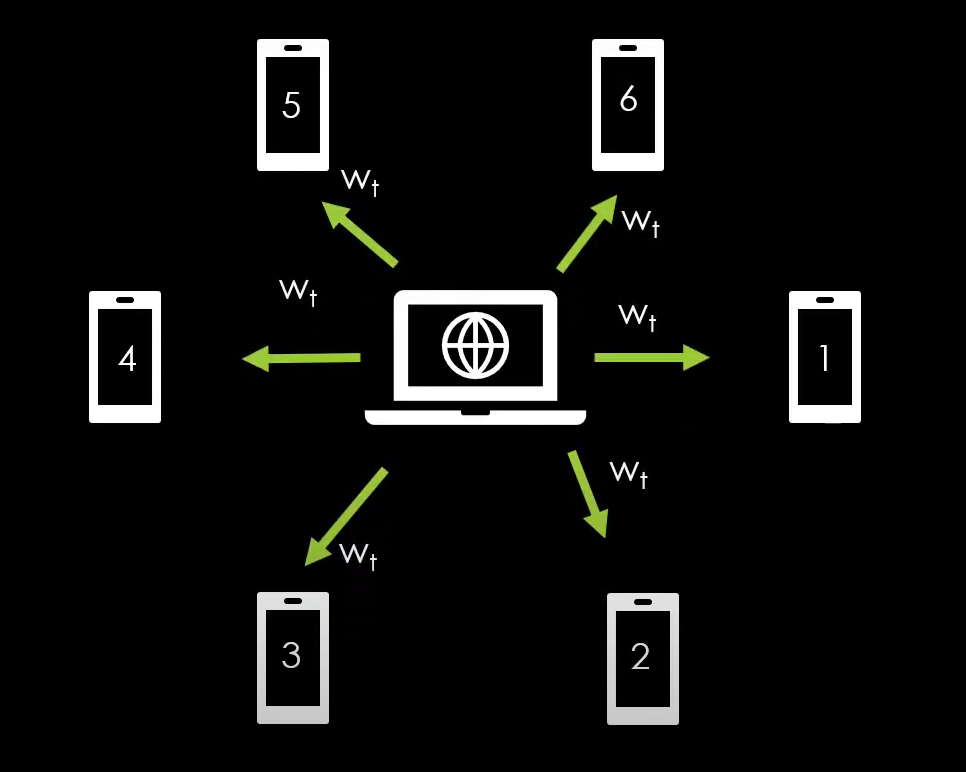
\includegraphics[width=1\textwidth]{fedavg_pic1.png}
			\end{minipage}
			\label{fig:grid_4figs_1cap_4subcap_1}
		}
		\subfigure[]{
			\begin{minipage}[b]{0.3\textwidth}
				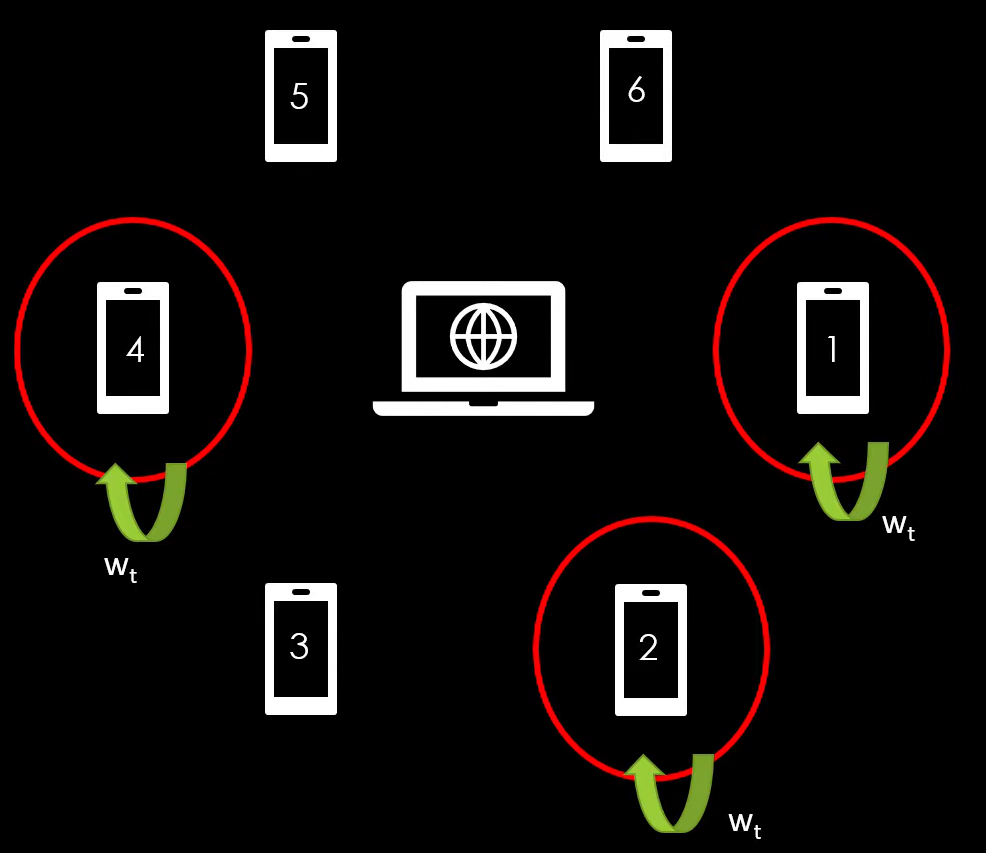
\includegraphics[width=1\textwidth]{fedavg_pic2.png}
			\end{minipage}
			\label{fig:grid_4figs_1cap_4subcap_2}
		}
		\\
		\subfigure[]{
			\begin{minipage}[b]{0.3\textwidth}
				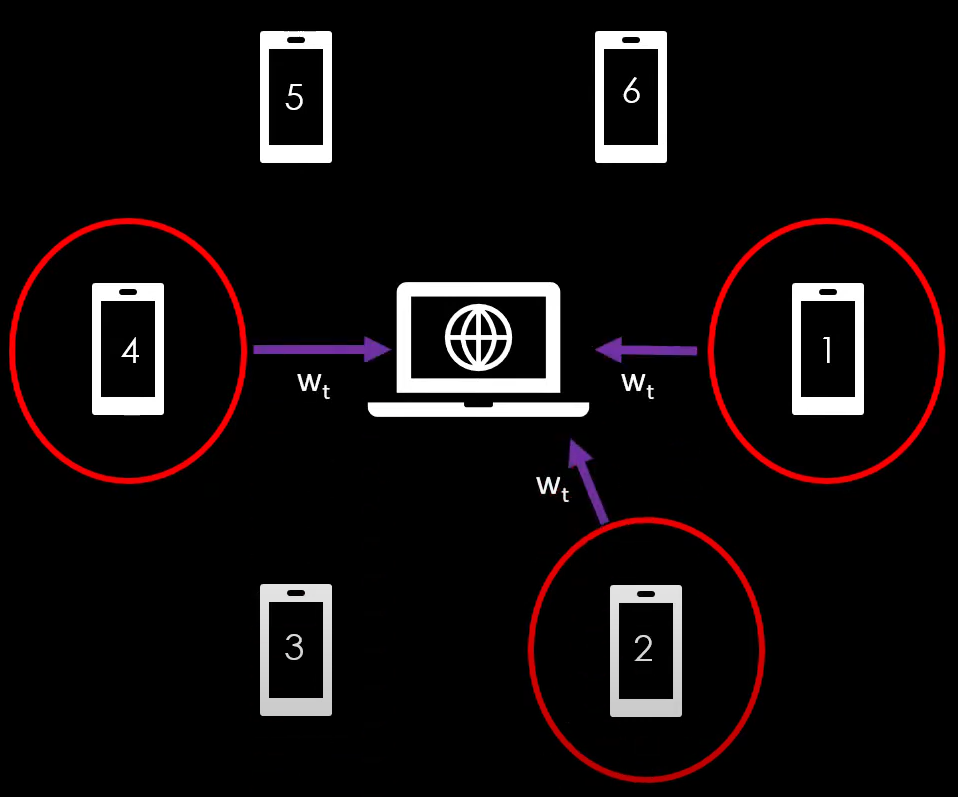
\includegraphics[width=1\textwidth]{fedavg_pic3.png}
			\end{minipage}
			\label{fig:grid_4figs_1cap_4subcap_3}
		}
		\subfigure[]{
			\begin{minipage}[b]{0.3\textwidth}
				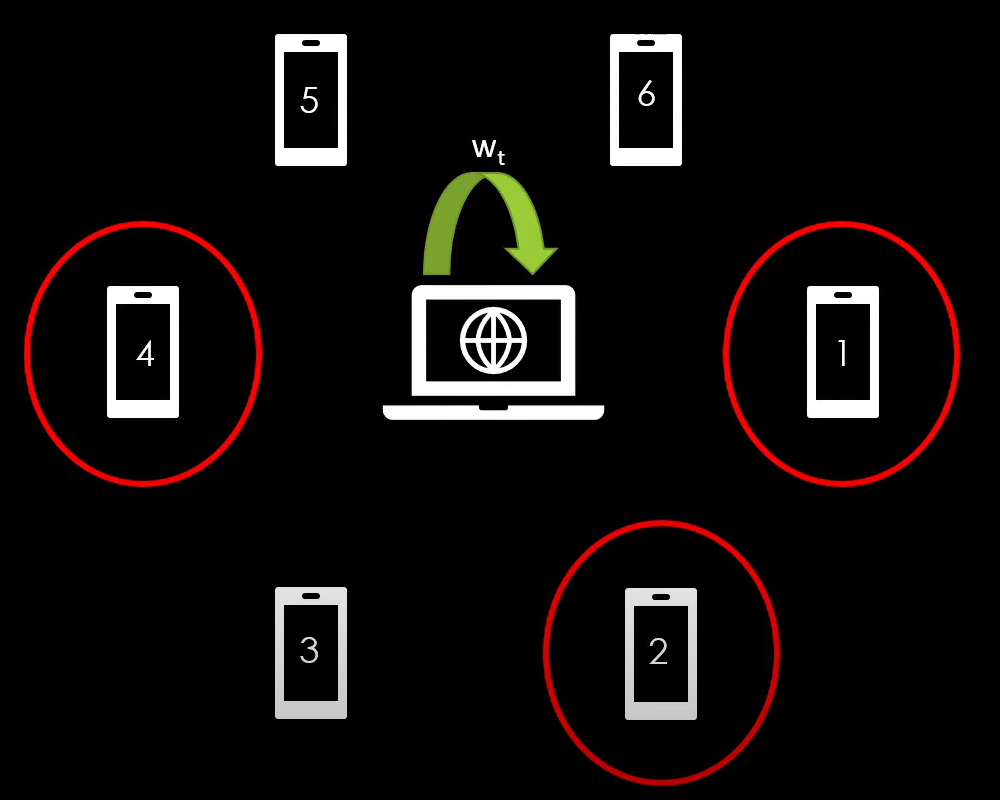
\includegraphics[width=1\textwidth]{fedavg_pic4.png}
			\end{minipage}
			\label{fig:grid_4figs_1cap_4subcap_4}
		}
		\caption{}
		\label{fig:grid_4figs_1cap_4subcap}
	\end{figure}
\end{frame}

\begin{frame}{Problem}
	There are two primary aspects of the algorithm;
	\begin{itemize}
		\item How to compute global/local loss function?
		\item How to compute global/local gradient calculation and update state
	\end{itemize}
\end{frame}

\begin{frame}{Objective Function}
	The objective function:
	\begin{align}
		\mathop{min}\limits_{\omega \in R^d}f(\omega)
	\end{align}
	\begin{align}
		f(\omega)=\frac{1}{n}\sum_{i=1}^{n}f_i(\omega)
	\end{align}
	Every client computes the loss function above with its local dataset
	Then these local loss scores are weighted-averaged
	\begin{align}
		f(\omega)=\sum_{k=1}^K\frac{n_k}{n}F_k(\omega)
	\end{align}

	\begin{align}
		F_k(\omega)=\frac{1}{n_k}\sum_{i \in P_k}^{n}f_i(\omega)
	\end{align}
\end{frame}

\begin{frame}{Optimize}
	\textbf{FederatedAveraging(or FedAvg)}\\
	Each client k locally takes one step of gradient descent on the global model with its local dataset.
	\begin{align}
		\forall k, \quad \omega_{t+1}\gets \omega_t-\eta g_k
	\end{align}
	Then the server takes a weighted average of the resulting models.
	\begin{align}
		\omega_{t+1}\gets \sum_{k=1}^{K} \frac{n_k}{n}\omega_{t+1}^k
	\end{align}
\end{frame}

\begin{frame}{Computation}
	(FedAvg) fits real world problems more.
	\begin{align}
		\omega^k \gets \omega^k-\eta \nabla F_k(\omega^k)
	\end{align}

	Computation is controlled by three key parameters for this approach
	\begin{itemize}
		\item C:The fraction of clients that perform computation  on each round.
		\item E:Number of training passes each client makes over its local dataset on each round.
		\item B:Local minibatch size used for the client updates.
	\end{itemize}
\end{frame}

\begin{frame}{Algorithm}

	\begin{figure}[htbp]
		\centering
		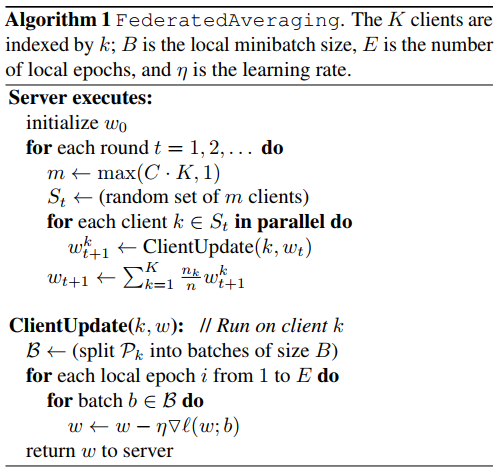
\includegraphics[scale=0.6]{alg.png}
		\caption{FederatedAveraging}
	\end{figure}
\end{frame}
\section{Experiments}
\begin{frame}{MNIST Digit Recognition}
	Model
	\begin{itemize}
		\item 2NN model\cite{lecun1998gradient}
		\item Basic CNN Model
	\end{itemize}
	Data distribution
	\begin{itemize}
		\item IID
		\item Non-IID
		      % \item 100 clients, each receiving 600 examples
	\end{itemize}


\end{frame}
\begin{frame}{The complete Works of William Shakespare}
	Model
	\begin{itemize}
		\item LSTM\cite{kim2016character}
	\end{itemize}
	Data distribution
	\begin{itemize}
		\item Balanced and IID version
		\item Unbalanced and non-IID version
	\end{itemize}
\end{frame}

\begin{frame}{Experiment Results}

	% \begin{table}[h!]
	% 	Increasing Computation per client
	% 	\begin{center}
	% 		\small
	% 		\caption{Your first table.}
	% 		\begin{tabular}{c|c|c|c|c|c} % <-- Alignments: 1st column left, 2nd middle and 3rd right, with vertical lines in between
	% 			\textbf{MINST 2NN} & \textbf{E} & \textbf{B} & \textbf{u} & \textbf{IID} & \textbf{Non-IID} \\
	% 			\hline
	% 			FEDSGD             & 1          & $\infty$   & 1          & 1468         & 1817             \\
	% 			FEDAVG             & 10         & $\infty$   & 10         & 156(9.4x)    & 1100(1.7x)       \\
	% 			FEDAVG             & 1          & 50         & 12         & 144(10.2x)   & 1183(1.5x)       \\
	% 			FEDAVG             & 20         & $\infty$   & 20         & 92(16.0x)    & 957(1.9x)        \\
	% 			FEDAVG             & 1          & 10         & 60         & 92(16.0x)    & 831(2.2x)        \\
	% 			FEDAVG             & 10         & 50         & 120        & 45(32.6x)    & 881(2.1x)        \\
	% 			FEDAVG             & 20         & 50         & 240        & 39(37.6x)    & 835(2.2x)        \\
	% 			FEDAVG             & 10         & 10         & 600        & 34(43.2x)    & 497(3.7x)        \\
	% 			FEDAVG             & 20         & 10         & 1200       & 32(45.9x)    & 738(2.5x)        \\
	% 		\end{tabular}
	% 	\end{center}
	% \end{table}
	\begin{figure}[htbp]
		\centering
		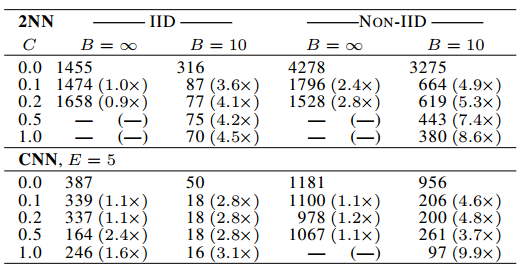
\includegraphics[scale=0.7]{table1.png}
		\caption{Effect of the client fraction C on the MNIST 2NN
			with E = 1 and CNN with E = 5.}
	\end{figure}
	C is set to 0.1 for all experiments. \\
	Computation increased by increasing E, decreasing B.
\end{frame}

\begin{frame}{Experiment Results}
	\begin{figure}[htbp]
		\centering
		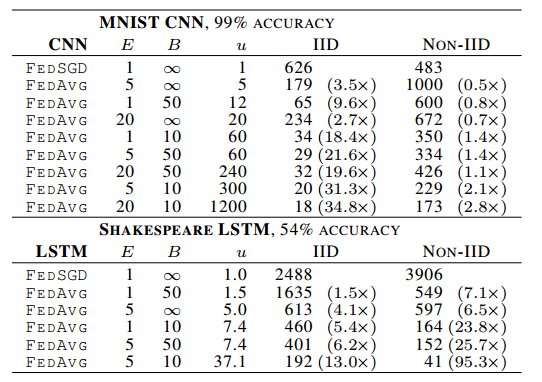
\includegraphics[scale=0.7]{table2.png}
		\caption{Effect of the client fraction C on the MNIST 2NN
			with E = 1 and CNN with E = 5.}
	\end{figure}
\end{frame}

\begin{frame}{Experiment Results}
	\begin{figure}[htbp]
		\begin{minipage}{0.6\textwidth}
			\centering
			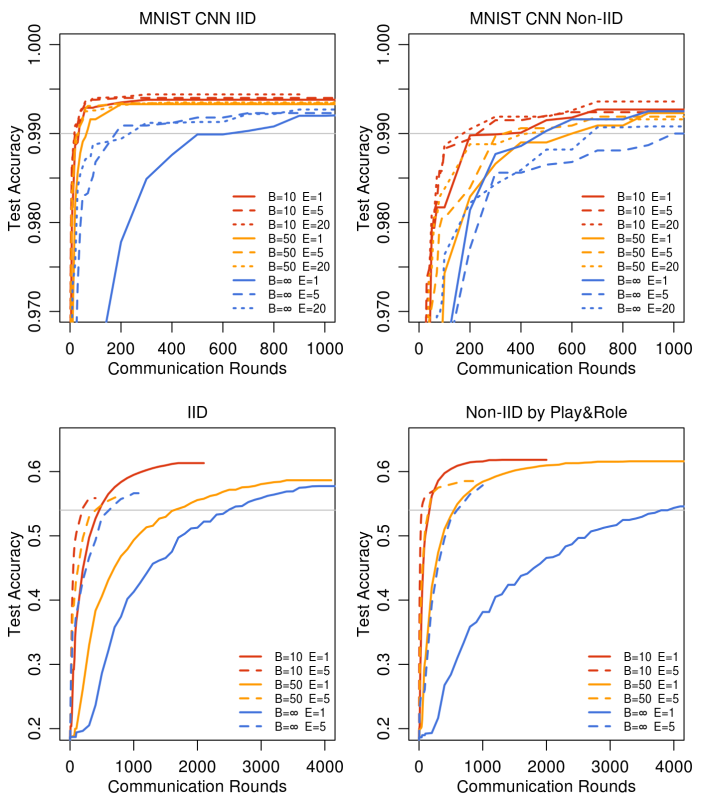
\includegraphics[scale=0.4]{line1.png}
		\end{minipage}%
		\hfill
		\begin{minipage}{0.4\textwidth}
			\caption{Test set accuracy vs. communication rounds
				for the MNIST CNN and Shakespeare LSTM  with
				C = 0.1 and optimized η. The gray lines show the target
				accuracies used in Table 4. }
		\end{minipage}
	\end{figure}
\end{frame}
\begin{frame}{Experiment Results}
	\begin{figure}[htbp]
		\centering
		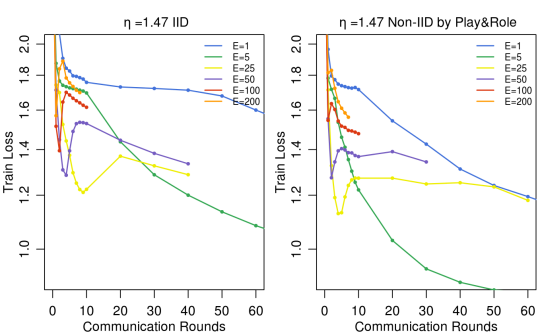
\includegraphics[scale=0.7]{table3.png}
		\caption{The effect of training for many local epochs between averaging steps, fixing B = 10 and C = 0.1 for
			the Shakespeare LSTM with a fixed learning rate η = 1.47.}
	\end{figure}
\end{frame}

\begin{frame}{Experiment Conclusion}
	\begin{itemize}
		\item Using extreme non IID data to train the model, FedAvg can also perform better than FedSGD, indicating that the FedAvg algorithm may have strong robustness.
		\item FedAvg has higher accuracy than FedSGD on the test set, and the author speculates that FedAvg produces a dropout like regularization effect.
		\item When larger, the accuracy of FedAvg algorithm convergence will decrease, or even not converge.
	\end{itemize}
\end{frame}

\section{Conclusion}
\begin{frame}{Conclusion}
	Fedavg trains high-quality models using relatively few rounds of communication.

	It offers many practical privacy benefits;

	\begin{itemize}
		\item Differential privacy
		\item Secure multi-party computation
	\end{itemize}
\end{frame}

\section{References}

\begin{frame}[allowframebreaks]
	\bibliography{ref}
	\bibliographystyle{njupt}
\end{frame}

\begin{frame}
	\begin{center}
		{\Huge \calligra Thanks!}
	\end{center}
\end{frame}

\end{document}